\documentclass{sig-alternate}

\usepackage{color}
\usepackage{cite}
\usepackage{float}
\usepackage{xspace}
\usepackage{amsfonts}
\usepackage{graphicx}
\usepackage{pgfgantt}
\usepackage{setspace}
\usepackage{gensymb}
\usepackage{pdfpages}
\usepackage{eurosym}
\usepackage{booktabs}
\usepackage{hyperref}
\usepackage[toc,page]{appendix}
\usepackage{multirow}

\hypersetup{
	colorlinks,
	citecolor=black,
	filecolor=black,
	linkcolor=black,
	urlcolor=black
}

\begin{document}

\title{Telemetry-based Optimisation for User Training in Racing Simulators}

\numberofauthors{1} 
\author{
	\alignauthor
	Fran\c{c}ois Buhagiar\\
    \email{francois.buhagiar.12@um.edu.mt}
}

\maketitle
\begin{abstract}

\end{abstract}

\keywords{Sim Racing, Motorsport Training, Serious Games}

\section{Introduction}

\section{Background work} {
\label{sec:background}

\subsection{Motorsport Racing}
In circuit motorsport racing, motorised vehicles go round a course for a set number of times. There are varies racing disciplines or series, each one having its own specific rules. However, at the core, participants in all disciplines aim to complete a full lap of the circuit in the shortest time. This paper will focus on one such discipline, that of confined car racing, which takes place on smooth asphalt surfaces in purpose-built race tracks in which the aim is to perform the fastest lap possible. 

\begin{figure}[!htb]
	\centering
	\begin{minipage}{0.45\textwidth}
		\centering
		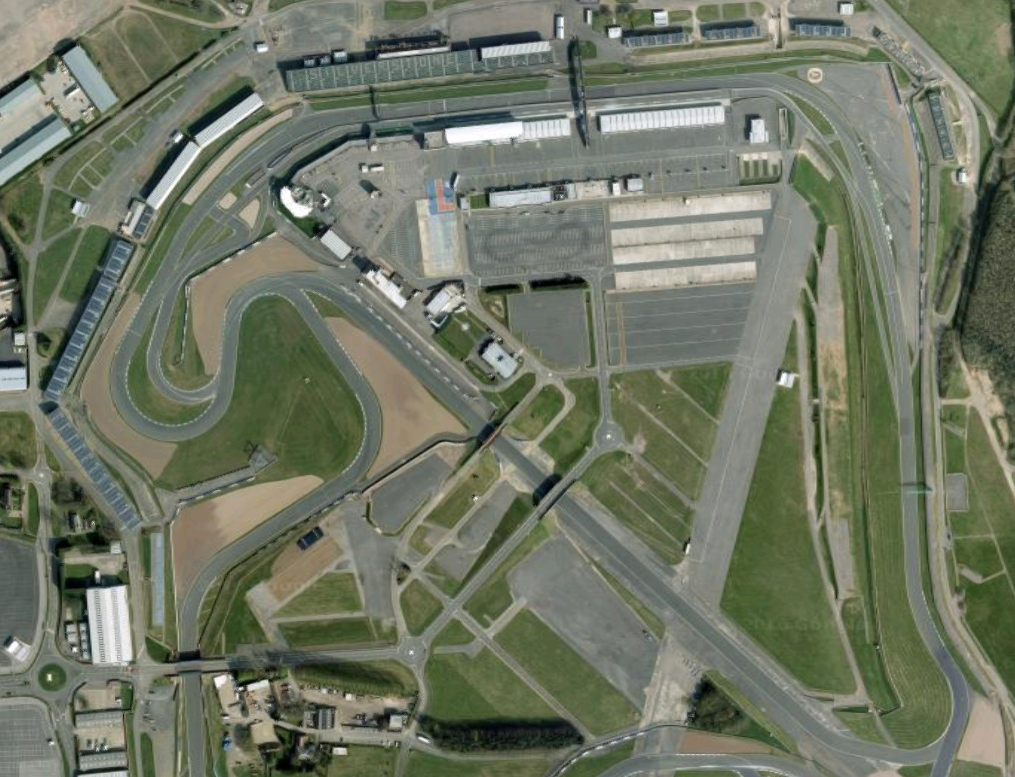
\includegraphics[width=\textwidth]{images/confinedCircuit}
		\caption{Example of confined car racing circuit}
		\label{fig:circuit-overhead}
	\end{minipage}\hfill
\end{figure}

\subsection{Racing Line}
\emph{A race driver needs to figure out how to go round a piece of asphalt in the minimum amount of time} \cite{GoingFaster}. In order to do so, he or she needs to develop techniques for more advanced vehicle control. One such technique is that of mastering the racing line, which is considered the fundamental skill a race driver must understand and master before moving on to anything else \cite{GoingFaster}. The racing line is the best path through a circuit: if followed, it is the path that yields the shortest time at the highest average speed \cite{beckman1991physics}. The trickiest part in achieving this is to master the racing line of a corner. Corners are split in three sections. The first section is the breaking part, where the car needs to sufficiently decelerate in preparation for the  \emph{turn-in point}. Thus, the second partition of the racing line at a corner is the segment between the turn-in point and the apex point, which is the inside mid-point of the corner (see Figure \ref{fig:CornerRaceLine}). After the turn-in point, the driver aims for the apex point. The final section of the racing line in a corner lies from the apex point onwards, where the driver must gradually accelerate out of the corner, while still turning, aiming for the outside apex (see Figure \ref{fig:CornerRaceLine}.

\begin{figure}[!htb]
	\centering
	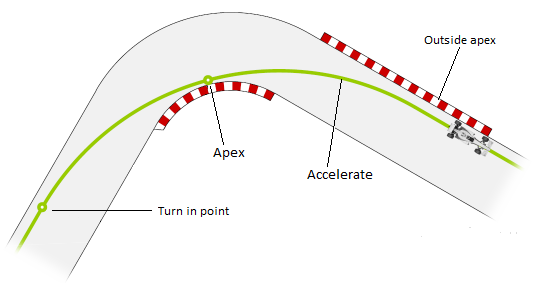
\includegraphics[width=0.45\textwidth]{images/cornerraceline}
	\caption{Racing line through a 90" right corner}
	\label{fig:CornerRaceLine}
\end{figure}

\subsection{Limit Of The Car}
After the driver develops a good grasp of the racing line, the limit of the car must be found. This is the highest speed the car can be driven while still retaining some measure of control. Various studies have been carried out to define such a limit in terms of the physical properties of the car and its environment \cite{beckman1991physics}. The most important property is the level of grip the car can achieve and sustain on track. A number of factors contribute to the level of grip. Most notably, one very important factor is the tyres as they are the only contact the car makes with the track, and allow for braking, accelerating and turning forces to be transferred to the asphalt.

Each tyre has two properties which are of particular interest: the slip ratio and slip angle. The slip ratio refers to the level of slip occurring between tyre rotational velocity and the asphalt which occur during acceleration and deceleration The \emph{slip ratio} is expressed as a percentage: a slip percentage of 100\% means that the tyre is rotating but the road is stationary. In jargon, this is called \emph{wheel spin}. On the other hand, a percentage of -100\% indicates that the tyre is not rotating but the road beneath is moving. This can occur when braking too hard and is called \emph{locking the wheels}. Both events need to be avoid by the driver as they not only put excessive wear and tear, they also impact negatively the performance of the driver. For an optimal braking procedure, the slip ratio should be between 10\% to 15\% \cite{GoingFaster} and no slip should occur during acceleration.

The slip angle is the angle between the tyre's desired direction (perpendicular to the axis of rotation of the tyre) and the tyre's actual direction (the direction the car is moving in). Given both the actual direction of travel ($\mathbf{d}_t$) and the desired direction ($\mathbf{d}_d$) are known, the slip angle $s_a$ is calculated as follows:
\begin{equation}
s_a = \cos^{-1}(\hat{\mathbf{d}}_d \cdot \hat{\mathbf{d}_t}),
\end{equation}
\noindent where $\hat{\mathbf{d}_d} = \frac{\mathbf{d}_d}{|\mathbf{d}_d|}$ and $\hat{\mathbf{d}_t} = \frac{\mathbf{d}_t}{|\mathbf{d}_t|}$ are the normalised direction vectors for desired and travel directions respectively.

Whenever the slip angle is above $0\degree$ ($s_a > 0$) the tyre is said to be in an understeering situation. Understeer can be caused by active factors such as cornering speed, throttle application, braking, steering inputs and weight transfer. A tyre has an optimal slip angle at which grip is maximised during cornering. The optimal slip angle for a road tyre is about $5\degree$, whereas for a slick tyre, which is purposely constructed for racing, is about $8\degree-10\degree$ \cite{beckman1991physics}.

An oversteering situation may arise from lack of grip; while understeer is caused by a lack of grip in the front tyres, oversteer is cause by a lack of grip on the rear tyres. Oversteer is usually denoted by the rear of the vehicle becoming unstable resulting in its rotation such that the driver is facing towards the inside of the corner. Similarly to understeer, the active factors causing oversteer are also cornering speed, throttle application, braking, steering inputs and weight transfer. Oversteer is usually induced by braking during a corner or accelerating too hard in a rear wheel drive vehicle.

\subsection{Telemetry Data}
In motorsport, telemetry data contains measurements of vehicle dynamics from the engine and other components and is transmitted to receiving equipment for remote monitoring. These measurements can serve to monitor and reconstruct the vehicle state at a particular point in time. Telemetry data in motorsports usually accounts for measurements of speed, engine speed, component temperatures, slip angles, slip ratios, etc. Telemetry is widely regarded as the most important source of information by motorsports engineers; analysing this data can lead to a better understanding of the respective strengths and weaknesses of the car and the driver \cite{CarDataAnalysis}. In this work, we posit that through the real-time analysis of telemetry data, the pedagogical aspect of sim racing can be exploited to teach race driving to non experts.

\subsection{Racing Simulation Rigs}
The racing simulation rig (sim racing rig) is a piece of equipment designed to mimic the cockpit of a real-world car. The quality of a sim racing rig is dependent on its authenticity - how similar it is to a real-world car - and its build quality. These rigs come in various shapes, forms and sizes, from hangar-sized hydraulic-driven car chassis, that cost millions of Euro, to the more modest, built from off-the-shelf commodity hardware. Minimally, a rig should provide a steering wheel, seating and a display. More sophisticated rigs augment the user experience by employing gear shifters, and clutch, throttle and breaking pedals. The more advanced components are furnished with a force feedback mechanism, a form of haptic technology used to replicate the sense of touch by applying forces or vibrations, or motions to the user \cite{li2015can}.

\subsection{Video Games and Serious Games}
The main contrast between video games and serious games is the use of pedagogic activities which aim to educate or instruct knowledge or skill \cite{zyda2005visual} in serious games as opposed to the pure leisurely aspects of the video game. Pedagogy is given preference over the amusement value which in some cases might not be found in serious games \cite{zyda2005visual}. Serious games need to educate the player with a specific type of content, whereas videos games need to entertain the player with whatever; racing, puzzles, it does not really matter, as long as the player enjoys it\cite{Harteveld2007}. On the other hand, serious game designers have multiple objectives, they still need to create a compelling and fun game, but also an educating and realistic game. From this it follows that three aspects as essential for a serious game, fun, learning and validity \cite{Harteveld2007}. The serious game should make use of pedagogical methods and theories to ensure knowledge can be conveyed.
}
\section{Methodology}

\section{Design and Implementation}

\section{Evaluation}

\section{Conclusions}

\bibliographystyle{abbrv}
\bibliography{sigproc}

\end{document}
